%!TEX root = ../thesis.tex
%2-Tools for spectral analysis
% Reduction processes for NIR
% Additions to IRAF toolchain
% Problem with order tracing
%
% Wavelength Calibration
%    All detectors together
%    With stellar and ThAr lines???
% Telluric Correction


NIR Data reduction:
Extensive effort was made to reduce these spectra, comparing two different techniques.
- corrections
- NIR reduction stages.
- spectral artifacts
- correction of artifacts
Crires reduction
- ESO gasgano
- DRACS
- Post dracs stages
- hindsight 



\chapter{NIR spectroscopic reduction}  % Main chapter title
\label{cha:reduction} 

%----------------------------------------------------------------------------------------
%	SECTION 1
%----------------------------------------------------------------------------------------
The work of this thesis relies on the use of NIR spectra obtained by the CRIRES instrument. This chapter contains an overview of reductions steps undertaken, highlighting key effects present for CRIRES specifically, a comparison between reduction pipelines was preformed of model used and post reduction steps taken to make the spectra usable for the follow chapters.  

\section{NIR spectroscopy}
Specifics of NIR verse optical


NIR spectroscopy requires the use of CMOS detectors which are a different technology to the more commonly known CCD's. Their use is required in the NIR as the quantum efficiency (how well it measures photons) for CCD's although great for visible is poor in the NIR. CMOS detectors have a higher quantum efficiency in the NIR. 
\change(rearange/reorgaize this paragraph.)


\subsection{General reduction Concepts}
\label{subsec:nir_reduction}
\unfinished{Should this general stuff be an appendix? }

Focus on our observations

There are 3 main effects that need to be accounted for in NIR spectroscopy which influence the observations and calibrations taken. We briefly detail them here and how they are corrected for

\subsubsection{Dark Current}
The dark current is the detection of thermal elections on the detector, without any light falling on the detector. \fref{fig:dark_current} shows the master dark frame created from averaging three dark frames for the flats (3 seconds) and the observations (180 seconds) both on the same scale. A strong glow is observed in the bottom corners due to the presence of nearby amplifiers. The electrical components of the detectors themselves are creating a signal on the detector.
For the CRIRES detectors the dark current the per pixel is around 0.2-0.4\,(\(e^{-}\)\si{\per\second}), while the glow at the two corners is around \(\sim9000 / 180\approx50\)\,\(e^{-}\)\si{\per\second}.


\begin{figure}[h]
\centering
%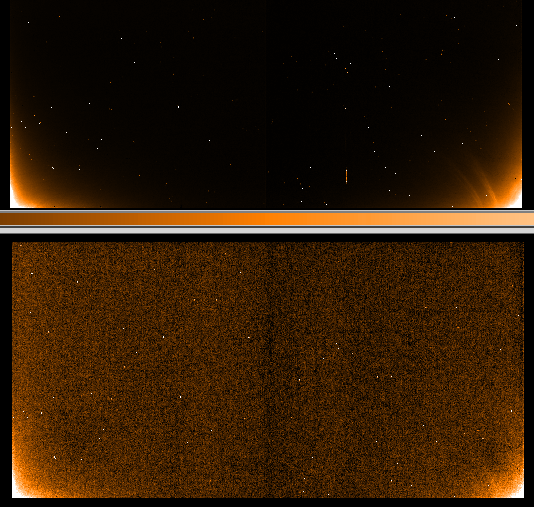
\includegraphics[width=0.4\textwidth]{figures/reduction/Master_Darks.png}
\includegraphics[width=0.9\textwidth]{figures/reduction/master_darks_1.pdf}
\caption{Master dark frame for 3 seconds and 180 seconds. Each created by averaging 3 Dark exposures at each setting. Both have been scaled to the maximum in the 180s exposure. The color is inverted so that black is the recorded measurement.}
\label{fig:dark_current}
\end{figure}


\subsubsection{Flat field}
To correct for pixel-to-pixel variations in sensitivity across the detector and for any distortions in the optical path a flat-field correction is needed. Exposures of a uniform light source are taken allowing the individual pixel-to-pixel sensitivity to be determined and corrected for. The flat field are corrected for dark current by subtraction of the master dark frame with the appropriate exposure time.

The CRIRES detector suffers from non-linearities in sensitivity across the detector. This can be seen in the flat field image on the left of \fref{fig:master_flats} where there is a gradient from white to black across the detector. A set of coefficients for each pixel is provided by ESO \footnote{Available at \href{https://www.eso.org/sci/facilities/paranal/instruments/crires/tools.html}{https://www.eso.org/sci/facilities/paranal/instruments/crires/tools.html}} to apply the correction for the non-linearity of the detectors. This also corrects for the odd-even affect observed in the CRIRES detectors in which there is a slight difference in output between the pixels from the odd and even columns. 

\begin{figure}[h]
    \centering
    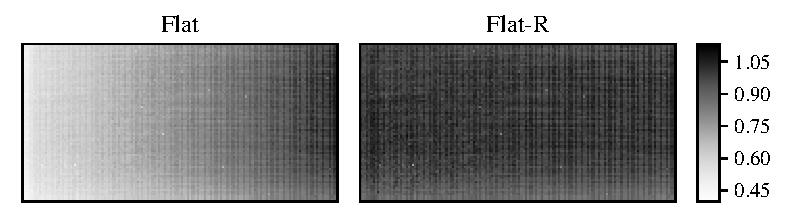
\includegraphics[width=0.9\textwidth]{figures/reduction/master_flats_1.pdf}
    \caption{A flat field image for a detector \#1 before (left) and after(right) the non-linearity corrections are preformed. A prefect detector would have all pixels in the flat field equal to 1.}
    \label{fig:master_flats}
\end{figure}


\subsubsection{Nodding and Jitter}
The technique of \emph{nodding} is used remove sky emission, detector dark current and glow. An observation is spit into multiple images. Between images the telescope is moved to shift target vertically in the slit. The light from the star travels through slightly different optical path and is recorded on a different part of the detector. The two nod positions A, B are then subtracted (A-B) to correct for the "non-target" measurement for each spectra.

An visual example of the nodding is shown in \fref{fig:nod_images}. On the left are \textbf{100?} pixel slices from the successive nod positions A and B as well as the difference A-B. On the right is a single pixel column from each image on the left. The background signal at the level of 20-30 counts in the image is almost canceled out by the opposite nod. This efficiently removes the background signal/noise from the observed spectra target. 

Observations of faint targets, that need long exposure times are also broken up into multiple images so that the instrument glow from \fref{fig:dark_current} does not saturate the detector.

\begin{figure}[h]
    \centering
    \begin{tabular}{cc}
   	 	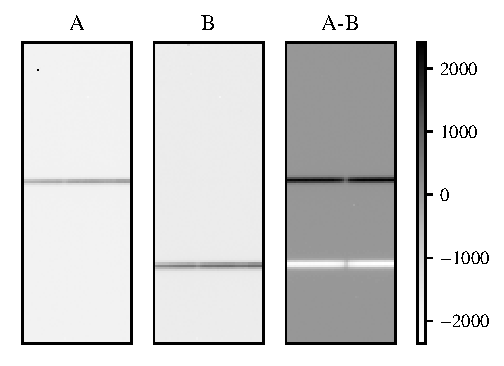
\includegraphics[width=0.4\textwidth]{figures/reduction/nod_image_sample.pdf} &
    	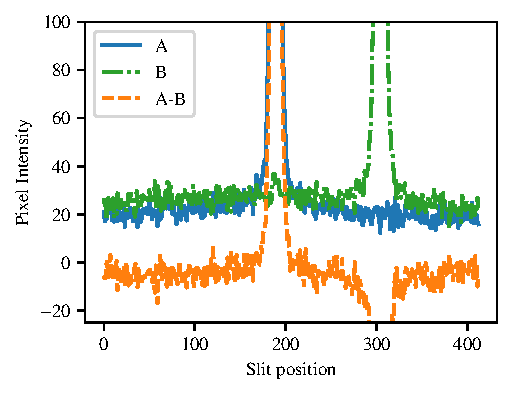
\includegraphics[width=0.37\textwidth]{figures/reduction/nod_slice_example.pdf}\\
    \end{tabular}
    \caption{Small section of nod position A, B and A-B for 1 HD30501 detector A. Right: A vertical slice  slice along the slit at position \textbf{512}.  The background is effectively removed by the subtraction of the orange}
    \label{fig:nod_images}
\end{figure}

\begin{figure}[h]
    \centering
    \caption{A}
	\label{fig:nod_slice}
\end{figure}

For each exposure at each nod position a \emph{jitter} is also be applied to allow the correction of bad pixels and decreases systematics of the detector. This is a small random vertical offset which ensures that all spectra at the same nod position do not consistently land on the same pixels each time.

\change{move}{As an example for the CRIRES observations analyzed here they were performed with a ABBAABBA nod cycle with a exposure time of 180s each, or 24 minutes all up.}



\subsection{TH-Ar Calibrations}\todo{Should I even include this section}
As part of the CRIRES calibration step there are images of Th-Ar lamp spectra from 6 fibers.

We didn't use as there are known issues in the NIR. (but this is what they look like??)

See other section \sref{subsec:wave_cal}.
\missingfigure{TH-AR exposure showing the few lines for calibration?}
Scratches on the detector often misidentified by eso pipline as th-ar lines.


\todo{Note: Useful information about MIR reduction in the 
\href{https://www.eso.org/sci/facilities/paranal/instruments/visir/doc/VLT-MAN-ESO-14300-3514_2018-02-01.pdf}{VISIR manual}}

%-----------------------------------
%	SUBSECTION 2
%-----------------------------------

\section{Pipeline Comparison}
To be able to extract the target spectra from the calibration and observation images a number of steps, some outlined above in \sref{subsec:nir_reduction}, have to be performed in sequence. The software tools that performs this series of steps is refereed to as a \emph{pipeline}. Each stage in the pipeline performs a specific task (e.g. average dark frame creation or nod subtraction), then passing it to the next stage. Two different pipelines were available to reduce the CRIRES observations use in this work. The first is the standard CRIRES pipeline\footnote{\href{https://www.eso.org/sci/software/pipelines/}{https://www.eso.org/sci/software/pipelines/}}, available from ESO.
The second is a in-house pipeline originally \change{was this the first instance} used in \citet{figueira_radial_2010} called DRACS (Data Reduction Algorithm for CRIRES Spectra) \change{Pedro it is my understanding that the ESO pipeline did not exist/was not available when you created DRACS, correct?}

In these next sections we document our experience using both pipelines, and compare the extracted spectra from both pipelines.


\subsection{CRIRES pipeline}
The spectra were initially reduced using the ESO CRIRES pipeline \href{ESO CRIRES pipeline}{ESO CRIRES pipeline}. The \href{https://www.eso.org/sci/software/gasgano.html}{GASGANO} graphical user interface (GUI) for the pipeline was used. The CRIRES reduction cookbook\footnote{\href{https://www.eso.org/sci/facilities/paranal/instruments/crires/doc/VLT-MAN-ESO-14200-4032\_v91.pdf}{https://www.eso.org/sci/facilities/paranal/instruments/crires/doc/VLT-MAN-ESO-14200-4032\_v91.pdf}} was followed to reduce the CRIRES nodding spectra. The CRIRES pipeline user manual\footnote{\href{ftp://ftp.eso.org/pub/dfs/pipelines/crires/crire-pipeline-manual-1.13.pdf}{ftp://ftp.eso.org/pub/dfs/pipelines/crires/crire-pipeline-manual-1.13.pdf}} and the the GASGANO manual\footnote{\href{here}{here}}. The pipeline provides a number of \emph{recipes} which preform the required extraction steps. From the GUI each recipe is manually selected, then the correct calibration and observation files are selected and added. 

- dark creation
- flat creation
- wavelength calibration
- jitter extraction

The wavelength calibration was the most tedious. To try and improve the wavelength calibration the y positions of the 6 Th-AR fibers was found for each detector and entered into the parameters for each observation. This sometimes helped but not always in the end we did not use them anyway.

The final output is a extracted and flattened spectra (although not normalized to 1) both in a rectangular and optimal and errors, with a wavelength calibration.

Opinions:
- For the extraction of many spectra it soon became tedious. Having to tweak parameters to obtain a better reduction. Then having to remember and change for each observation.  

 - Having the available options visible in the GUI for each spectrum is handy if you need to change them.

\todo{CONTINUE FROM HERE}

One good thing is it had the list of parameters available to tweak for that recipe visible..

It is believed that there is a way to enable 

It soon became tedious to use the Gasgano GUI to extract the many spectra reduce many and tweak all the parameter settings manually. In particular manually measuring and adding the vertical positions of the 6 Th-AR lines for each detector and observation. This was in an attempt to improve the wavelength calibration provided by the Th-AR lamp spectra.
A number of other parameters were tweaked from the defaults in an attempt to  improve the reduction. Again become tedious to repeatably change the parameters for all observations.

Having the GUI id however allow for a easy introduction into using performing spectral reduction when not of not yet comfortable with the command line (required for the ESOREX interface).
There is a command line interface available, ESOREX but it is not The newer ESO pipeline reduction tool Reflex does not have a pipeline for CRIRES. 


\subsection{DRACS}
DRACS (Data Reduction Algorithm for CRIRES Spectra) is custom reduction pipeline \citep{figueira_radial_2010} written in IRAF's CL\footnote{IRAF is distributed by the National Optical Astronomy Observatories, which are operated by the Association of Universities for Research in Astronomy, {Inc.}, under cooperative agreement with the National Science Foundation.} \citep{tody_iraf_1993}.  It provides for automated dark and non-linearity corrections (using the non-linearity coefficients provided by ESO), as well as the flagging and replacement of bad pixels. The images are corrected from sensitivity variations by dividing by a flat-field corrected from the blaze function effect. The nodding pairs are mutually subtracted and the order tracing is accomplished by fitting cubic splines
Order tracing allows the extraction algorithm to follow the shape for the dispersion across the detector.\footnote{The spectra do not fall perfectly horizontally on the detector and usually contain some curvature due to the instruments optics\todo{is this correct}{instruments optics}.}     
DRACS performs optimal extraction\citep{horne_optimal_1986} by default. 
By default the pipeline returns the optimal extraction \citep{horne_optimal_1986}.
Each extracted nod-cycle spectrum is then continuum normalized by dividing by a polynomial fitted to the continuum, with the polynomial degree selected for each spectrum and detector. Finally the normalized nod-cycle spectra are averaged together to give a single reduced spectrum, normalized to 1.

After the extraction of the individual nod spectra 
with some of the parameters altered to better suit the K-band instead of the H-band setting it was originally designed for

Opinions:
The DRACS can be run semi-autonomously so that it provides a consistent reduction relatively easily. It remembers the order tracing and 

How to use:
To use DRACS you need to create a number of lists with different, darks, flats, observations. \footnote{The GASGANO GUI was helpful to help identify the distinction of each fits file for a beginner}. A similar process with list of files is done with the ESOREX pipeline.
Once these list are created then the main script can be executed that semi-autonomously preforms the reduction. The first time though there are a number of manual checks/decisions, (e.g. confirming the order tracing position, and fit) but DRACS remembers them. This means the extraction requires less manual input if run a second or third time though.

This was handy when trying to tune some of the internal parameters to preform a better extraction.

\missingfigure{order tracing example plot?, exaggerated sketch} 

The most tedious thing about DRACS is creating the lists for the different input parameters

This semi-autonomous nature mean all the spectra are reduced in a consistent way and quickly, not requiring manual spectra selection for each observation.

At this point one would normally combine all the nod spectra together to improve the signal. However, we found that for some spectra the presence of cosmic rays or bad pixels heavily affected the variance weighting during the \emph{optimal} extraction. This caused noticeable extended artifacts in the extracted spectra of individual nods. An example of this can be seen in \fref{fig:nod_artifacts}. This created flux deviations in the combined optimally extracted spectra of \(\sim 0.5\% \).  Therefore, we took measures to remove these artifacts before combining the nod spectra as we are trying to recover companion spectra with expected flux ratios \(\rm {F_2}/{F_1} < 1\% \). 

The individual nod spectra that contained artifacts were visually identified by comparing all 8 nod spectra together, as shown in \fref{fig:nod_artifacts}, and also inspecting the difference between the mean and the median of the 8 nod spectra. The optimally extracted nods that contained artifacts (top panel) were replaced with their rectangularly extracted counter-parts (middle panel). An iterative 4-\(\sigma \) rejection algorithm\footnote{Found at \url{https://github.com/jason-neal/nod_combination}} was applied to the replacement rectangular extractions to remove the erroneous pixels that caused the artifacts. The \(\sigma\) value for each pixel was calculated as the standard deviation of the nearest 2 pixels on either side of all 8 nod spectra. The rejected pixels were replaced using linear interpolation.

For the remainder of the paper we use combined spectra constructed by averaging the 8 nod-cycle spectra together, where some of the optimally extracted spectra have been replaced using the above method. The last panel of \fref{fig:nod_artifacts} shows that the difference between the combined optimally extracted spectra and the \emph{combined extraction with replacements}.

\missingfigure{Example of an artifact in the optimally extracted spectra. The top panel contains the 8 normalized nod spectra after optimal extraction, while the middle panel shows the rectangular extraction for the exact same spectra. A vertical offset is included between each spectra. A single large spike in the seventh nod (pink) near pixel 230 creates a wide and noticeable artifact in the optimal extraction. The bottom panel shows the difference between a combined spectrum using the optimal nods only and a combined spectrum in which the seventh nod is replaced with its rectangular counterpart. The nod spectra are in observation order from top to bottom.}
% \begin{figure}
% 	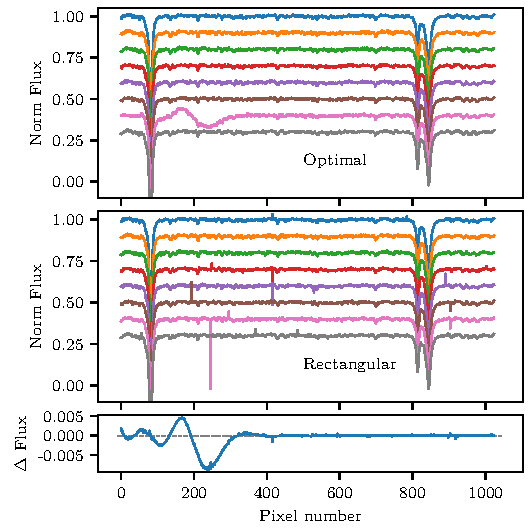
\includegraphics[width=\hsize]{images/final/Bad_pixel_replacement.pdf}  % chktex 8
% 	\caption{Example of an artifact in the optimally extracted spectra. The top panel contains the 8 normalized nod spectra after optimal extraction, while the middle panel shows the rectangular extraction for the exact same spectra. A vertical offset is included between each spectra. A single large spike in the seventh nod (pink) near pixel 230 creates a wide and noticeable artifact in the optimal extraction. The bottom panel shows the difference between a combined spectrum using the optimal nods only and a combined spectrum in which the seventh nod is replaced with its rectangular counterpart. The nod spectra are in observation order from top to bottom.}
% 	\label{fig:nod_artifacts}
% \end{figure}

\subsection{Reduction choice }

After both methods were used to reduce a number of spectra we compared the output to check the quality of each. One of the important things we checked was the line depth of the spectra. To insure that DRACS was comparable to the ESO pipeline.

We in-fact found they were the same line depth.


After using both it was decided to continue using DRACS ... for this reasons
. 
The main reason for both pipelines was to check the reduction output were similar, especially the line depths.
\missingfigure(spectra from both reduction methods to show similarities)

With these considerations at this point we decided to continue to use the DRACS pipeline. This would require our own wavelength calibration. 


BUT: We eventually found some strange inconsistencies in the DRACS reduction, artifacts. where bad pixels were non-optimally corrrected....
In hindsight it may have been better to use ESO (if a way to semi-automation was discovered)



\subsubsection{Reduction issues}

There are two types of extraction commonly used. The \emph{rectangular} extraction performs a rectangular aperture sum in the spatial direction while the \emph{optimal} extraction \citep{horne_optimal_1986} also includes variance weighting to reduce the impact of the noise and deviant pixels on the total flux measurement. Optimal extraction is the most common and is the default output of both the ESO and DRACS pipelines.

After choosing to continue using the DRACS pipeline it was later discovered that there were strong artifacts present in the reduced DRACS spectra, m
\missingfigure{Example artifacts}

Some time later it was noticed that some spectra had issues. these arose from the optimal extraction in the DRACS pipeline where bad pixels would cause removed


It could be that these are a incorrect bad pixel mask.

\missingfigure{Table of frames that were replaced} 
The normalization and nod combining steps were also performed using IRAF while the following post reduction procedures and analysis all utilize \emph{Python}. This pipeline was chosen over the ESO CRIRES pipeline because it seemed relatively simple to use, being mostly automated, and appeared to have less bad pixel/cosmic ray artifacts in the resulting spectra. In hindsight this was not the case, with artifacts appearing that needed to be removed. 

One possible explanation for the artifacts present is an instrumental effect, such as instrument glow. This is known to affect CRIRES and included in the data reduction cookbook \citep{smoker_very_2012}. These artifacts in the K-band spectra were not observed in previous works in the H-band using this pipeline and as such may have a wavelength dependent affect, as the higher wavelength nIR is more susceptible to thermal instrument glow.


\section{Reduction experience:}
The experience gained in reducing CRIRES spectra allowed for some collaboration in other works. The DRACS pipeline was used to extract the spectra of two other targets. A brief aim of each science case is given below.
\begin{itemize}
\item Barnard's Star\footnote{Programme ID: 085.D-0161(A)}: Reduced to extend the work of \citet{andreasen_nearinfrared_2016} in derivation spectroscopic parameters in the NIR. Unfortunately the reduced NIR spectra from the CRIRES-POP library was used instead in \citet{Andreasen et al. (in prep.)}. 
\item $\eta$ Tel\footnote{Programme ID: 083.C-0759(A)}: To measure the rotation rate of the a quickly rotating Brown Dwarf by measuring the line broadening. \change{}{Hagelberg et al. (in prep.)}
\item The spectra of $\eta$ Tel was also used to compare different telluric correction methods in \cite{ulmer-moll_telluric_2018}.
\end{itemize}

For these works only the spectral extraction outlined above was performed. The post \change{I seem to use these interchangeably. are they}{extraction/reduction} steps from the following sections were not.

\missingfigure{An image of some reduced spectra from eta Tel and Barnard's star???}


\section{Post reduction stages}
\label{sec:posreduction}
After using DRACS we have an extracted 1-D spectra of the target. The spectra has had wavelength information added yet or been corrected for telluric lines. We will address these two things in the following section.

\subsubsection{Wavelength calibration}
\label{subsec:wave_cal}
Wavelength calibration, assigning accurate wavelength values to each pixel in the spectra, is challenging in the NIR with CRIRES. CRIRES uses a Thorium-Argon (Th-Ar) lamp to place 6 emission spectra on the detector using fibers. The spectra of the Th-AR emission lines are used to determine the spatial distribution of the wavelength solution across each detector. \change{fix-up get a good citation, number of lines}{Th-Ar lamps are excellent at optical wavelengths where their numerous (8600 espresso) spectral lines enable precisions of sub-m/s HARPS spectrograph\cite{paper}}. However in the NIR, there is a low density of Th-Ar lines \citep{kerber_laboratory_2009}, which, in combination with the alignment of the narrow wavelength range of the detector, causes a poor wavelength calibration to be obtained (e.g.\ CRIRES-POP \citep{nicholls_crirespop_2017})
We experienced these issue ourselves when using the ESO CRIRES pipeline. At the wavelength of 2.1-2.7 micron there are roughly XXX th-ar lines across the detectors.
The calibration with the ESO pipeline recipes often would provide poor The DRACS pipeline does not use the Th-AR lamp files for wavelength calibration and leaves it for post reduction analysis

The crires manuals point out that above 2.2 micron there are O-H sky lines that can be used for calibration but we focus at 2.1-2.2 where we are they are too dim.
 
Therefore, we use the telluric absorption lines present in each observation as the wavelength reference. Instead of directly using the HITRAN database \citep{rothman_hitran2012_2013} for the line positions of the telluric spectra (e.g.~\citep{brogi_signature_2012,brogi_carbon_2014,dekok_detection_2013}), we use TAPAS atmospheric transmission models \citep{bertaux_tapas_2014} obtained for each observation. These in turn use the HITRAN database but include atmospheric profiles and physical measurements to model the telluric absorption strength.

The centroid of each telluric line is obtained by fitting the telluric transmission spectrum, \(T \), as a sum of Gaussian functions (subtracted from the continuum) representing the telluric lines,

\begin{equation}
T(\lambda) = 1 - {\Sigma}_{i}\ G(\lambda, A_{i}, {\mu}_{i}, {\sigma}_{i}),
\end{equation}

where \(G \) is a Gaussian function of the form

\begin{equation}
G(\lambda, A, \mu, \sigma) = {A \textrm{e}}^{{-(\lambda-\mu)}^{2}/2\sigma^{2}}
\end{equation}

and \(A \), \(\mu \), \(\sigma \) are the amplitude, central wavelength, and standard deviation for each line respectively. Telluric lines actually have a \todo{Mention somewhere what a voigt profile is. convolution of Gaussain and Lorentzian (thermal verse pressure broadening)} Voigt profile but at this resolution the Gaussian profile dominates, and as such the Gaussian assumption is a good one for the fit to find the line centers.

The observed spectra contain two different components: stellar and telluric lines overlapped. This overlapping is, in fact, a multiplication of the stellar and telluric spectra. These were fitted with two Gaussian-sum models multiplied together, with the identification of telluric and stellar lines performed manually for each spectra, using the synthetic telluric models as the reference.
\begin{align}
I_{obs}(x) &= I_{tell}(x) \times I_{space}(x) \nonumber \\
I_{obs}(x) &= \Big(1 - {\Sigma}_{j}\ G(x, A_{j}, {\mu}_{j}, {\sigma}_{j})\Big) \times \Big(1 - {\Sigma}_{k} G(x, A_{k}, {\mu}_{k}, {\sigma}_{k})\Big), \label{eqn:obs}
\end{align}

where \(x \) is the pixel coordinate of the extracted spectra.

The wavelength solution was obtained by fitting a second order polynomial, shown to be sufficient for higher precision RV studies \citep[e.g.][]{bean_groundbased_2010, figueira_radial_2010}, to the centroid values \(\{\mu(x), \mu(\lambda)\} \) obtained from the telluric component of the observed spectra and telluric model respectively. 

Much like issues with Th-Ar calibrations this method only works well when there is sufficient coverage of telluric lines on the detector. For the wavelength setting of these observations, the spectra from the second detector (top right panel of \fref{fig:detector4allspectra}) only have two large telluric lines present with several small lines, with relative depths smaller than 1\%, which are difficult to identify. This deteriorated the calibration stability for the second detector. With the lack of telluric contamination and stellar lines on the second detector it may have been ideal for the detection of a faint secondary spectra; unfortunately the wavelength calibration quality varies in an inverse way.

We note that there are many variations on this wavelength-calibration technique including those integrated within programs such as TelFit \citet{gullikson_correcting_2014}, and ESOs Molecfit \citet{smette_molecfit_2015}, that perform telluric correction and re-calibrate the wavelength axis themselves.


\unfinished{Add pictures of wavelength calibrations}

\missingfigure{Extracted, normalized and wavelength calibrated spectra for a single observation of each target. The target name is given above each spectrum along with the observation number. Each panel is the spectra from a single detector 1--4 in order of increasing wavelength. The black dashed lines indicate the unique telluric spectrum used for wavelength calibration and telluric correction for each observation.}
% \begin{figure*}
% 	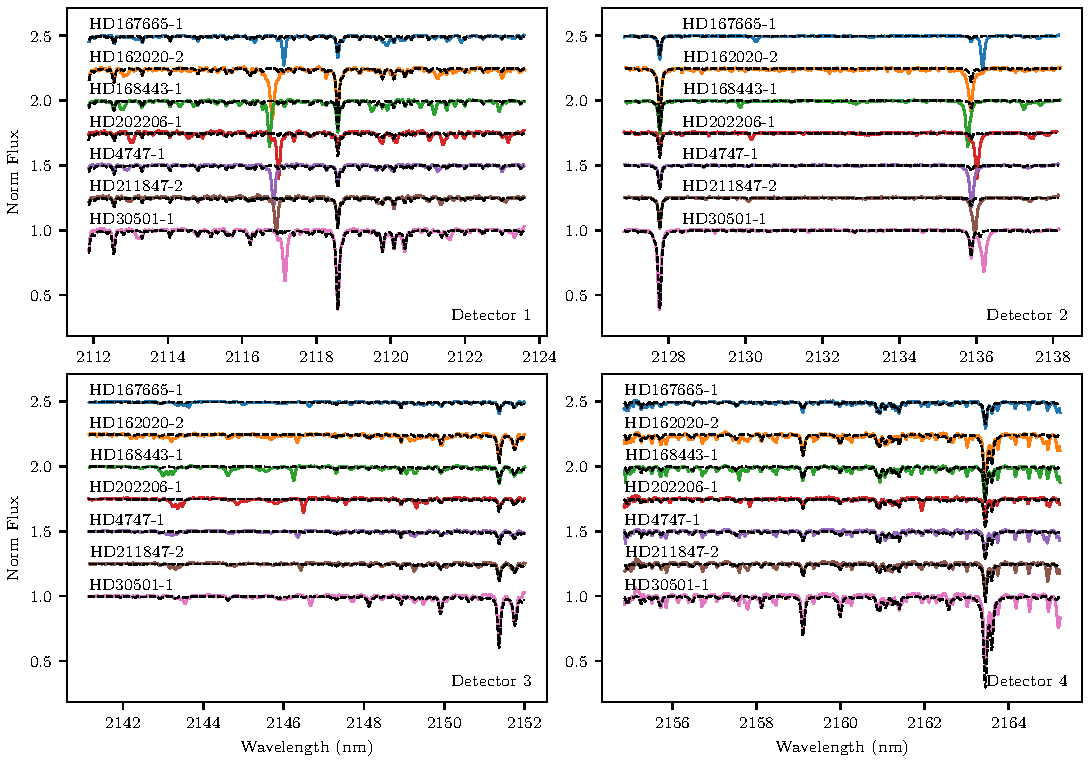
\includegraphics[width=\hsize]{figures/reduction/Spectra_examples.pdf}
% 	\caption{Extracted, normalized and wavelength calibrated spectra for a single observation of each target. The target name is given above each spectrum along with the observation number. Each panel is the spectra from a single detector 1--4 in order of increasing wavelength. The black dashed lines indicate the unique telluric spectrum used for wavelength calibration and telluric correction for each observation.}
% 	\label{fig:detector4allspectra}
% \end{figure*}



\unfinished{See Solene's paper regarding Telluric correction with models and reference spectra}

Telluric Correction:
TAPAS
Requiring data from tapas
- not handy for many
- own script to derive from spectra header.


\subsubsection{Telluric correction}
\label{subsec:telluric_correction}
Ground based observations require the removal of the absorption lines introduced by Earth's atmosphere. These observations were first taken in an atmospheric window of the K-band in order to reduce the absorption introduced by the atmosphere \citep{barnes_hd_2008}. To correct for the remaining telluric line contamination the spectra were divided by the TAPAS\citep{bertaux_tapas_2014} atmospheric transmission models for each observation. Synthetic telluric models were used to avoid the observing overhead necessary to perform telluric standard star exposures \citep{vacca_method_2003}, and they have been demonstrated to be superior in the quality of the correction relative to the telluric standard approach \citep[e.g.][]{cotton_atmospheric_2014}.

Before the correction, the depth of the telluric lines were re-scaled to match the airmass of the observation using the relation \(\rm T = T^{\beta} \), where \(\rm T\) is the telluric spectrum and \(\beta \) is the airmass ratio between the observation and model. This changed the depth of most absorption lines to match the observations, but does not correctly scale the deeper \(\rm H_{2}O \) lines. The scaled telluric model is interpolated to the wavelengths of the observed spectrum and then used to correct the observed spectra through division, leaving behind a telluric corrected spectra. An example of a telluric corrected spectra is shown in the middle panel of \fref{fig:spectral_example}, with the light blue shading indicating where the deeper telluric lines were.

We attempted the technique suggested by \citet{bertaux_tapas_2014} to address the poor \(\rm H_{2}O \) airmass scaling, to fit a scaling factor to the \(\rm {H}_{2}O \) absorption lines before convolution to the instrument resolution. This was achieved by first dividing the spectrum by a telluric model with only non-\(\rm H_{2}O \) constituents, convolved to the observed resolution, and scaled by the airmass to remove the non-\(\rm H_{2}O \) lines. Then a model with only \(\rm H_{2}O \) lines at full resolution was scaled by a factor \(\textrm{T}^{x} \), convolved to \(\rm R=50\,000 \) and compared to the observed spectra. The factor \(x \) was fitted to find the best scaling factor for the \(\rm H_{2}O \) lines.

We found that for a few spectra in our sample this method corrected the deeper telluric lines well, but in many cases we found that the fitted scaling factor was affected by the presence of blended stellar lines (attempting to fit those also). It was also strongly influenced by the deepest \(H_{2}O\) telluric lines present. We find that the telluric correction of the deep \(\rm H_{2}O \) lines could be improved with this technique, but, at the cost of worsening the correction of the many smaller \(\rm H_{2}O \) lines. Since the smaller \(\rm H_{2}O \) lines covered more of the spectrum in this region than the larger lines we chose not to continue with this separate \(\rm H_{2}O \) scaling. One possible solution for this would be to perform a piece-wise telluric correction, performing this step only for the deeper \( \rm H_{2}O\) lines, or by using one of the other tools that fits the telluric model to the observations. This technique could also benefit from a larger wavelength span that would enable blended lines to be ignored while having sufficient deep \(\rm H_{2}O\) lines to fit the scaling factor correctly. This small experiment shows that a simple scaling is not enough to correct for the absorption in an effective way, for this case.

\unfinished{Add telluric spectra for NIR band? the plot from Molecfit?}

\unfinished{Still uneven line coverage on all detectors in this small range}

\unfinished{H\_2\_0 corrections}  example of good and bad fitting...


\subsection{Tapas models}
\label{subsec:tapas_models}
We used telluric line models to wavelength calibrate the reduced spectra in \sref{subsec:wave_cal} and to correct for the atmospheric absorption in \sref{subsec:telluric_correction}. We utilized the TAPAS (Transmissions of the AtmosPhere for AStronomical data) web-service\footnote{\url{http://www.pole-ether.fr/tapas/}} \citep{bertaux_tapas_2014} to obtain atmospheric transmission models for each observation. TAPAS uses the standard line-by-line radiation transfer model code LBLRTM~\citep{clough_linebyline_1995} along with the 2008 HITRAN spectroscopic database~\citep{rothman_hitran_2009} and Arletty atmospheric profiles derived using meteorological measurements from the ETHER data center\footnote{\url{http://www.pole-ether.fr}}, which has a 6 hour resolution in atmospheric profiles.
We use the mid-observation time to retrieve transmission models for each observation, with the Arletty atmospheric profiles\footnote{Nearest of the 6 hourly profiles} and vacuum wavelengths. The telluric models were retrieved without any barycentric correction to keep the telluric lines at a RV of zero with respect to the instrument. We obtained one model with all provided species present, convolved to a resolution of \(\rm R=50\,000 \), and another two models without an instrumental profile convolution applied. For these two extra models, one contained only the transmission spectra of \(\rm H_{2}O \) while the other was for all other constituents except \(\rm H_{2}O \). This was to explore a known issue \citep{bertaux_tapas_2014} with the depth of \(\rm H_{2}O \) absorption lines in \sref{subsec:telluric_correction}.

After the telluric correction is performed, the spectra are corrected for Earth's barycentric RV using PyAstronomy's\footnote{https://pyastronomy.readthedocs.io} \emph{helcor} function ported from the REDUCE IDL package (See \citet[][]{piskunov_new_2002}).



The telluric spectra from TAPAS can not only be used for correcting individual spectra but are also easily used to create a wavelength mask of deep telluric lines. For instance \citet{figueira_radial_2016} and \citet{artigau_optical_2018} use TAPAS spectra to mask out atmospheric lines deeper than 2\% for the computation of photon noise precision of radial velocity measurements. 



\todo{Look at } -> synthesizing telluric spectra NIR for CRIRES \cite{seifahrt_synthesising_2010}


Using TAPAS is contrasted alongside Molecfit and Tellfit in \cite{ulmer-moll_telluric_2018}. We conclude that....

\subsection{Wavelength masking}
Throughout the course of this work we found regions of the spectra found several regions from which we cannot reliably extract information.
We apply masks to these areas to remove them from the spectra. We collate the main reasons for the wavelength masking below 

Firstly, regions near the edges of each detector where the wavelength solution is extrapolated outside of the calibrating telluric lines are removed, reducing the effective size of each detector by about \(10\%\) or \(\sim100\) pixels. 

Secondly, we mask out any remaining artifacts present in the spectra and the centers of deep telluric lines where telluric correction was not corrected properly, sometimes resulting in "emission-like" peaks in the corrected spectrum. These factors combined result in masking out around a further 10\% of the observed spectra. 

In ~\sref{sec:results} we also apply a further wavelength restriction to mask out regions where there is a large mismatch between the observed spectrum and the closest synthetic spectra to the host. This significantly restricts the wavelength span utilized for that purpose to around only 43\% and the masked regions are visible in \fref{fig:visualinspection-hd2118471}. 


\unfinished{ADD non/H20 fitting corrections.}

\missingfigure{Plots showing some examples the telluric correction with and without H20 separated}

